%%%%%%%%%%%%%%%%%%%%%%%%%%%%%%%%%%%%%%%%%%%%%%%%%%%%%%%%%%%%%%%%%
% MUW Presentation
% LaTeX Template
% Version 1.0 (27/12/2016)
%
% License:
% CC BY-NC-SA 4.0 (http://creativecommons.org/licenses/by-nc-sa/3.0/)
%
% Created by:
% Nicolas Ballarini, CeMSIIS, Medical University of Vienna
% nicoballarini@gmail.com
% http://statistics.msi.meduniwien.ac.at/
%
% Customized for UAH by:
% David F. Barrero, Departamento de Automática, UAH
%%%%%%%%%%%%%%%%%%%%%%%%%%%%%%%%%%%%%%%%%%%%%%%%%%%%%%%%%%%%%%%%%

\documentclass[10pt,compress]{beamer} % Change 10pt to make fonts of a different size
\mode<presentation>

\usepackage[spanish]{babel}
\usepackage{fontspec}
\usepackage{tikz}
\usepackage{etoolbox}
\usepackage{xcolor}
\usepackage{xstring}
\usepackage{listings}

% Custom packages
\usepackage{standalone}
\usepackage{multicol}
\usepackage{multirow} % Confusion matrix
\usepackage{tikz}
\usepackage{pgfplots}
\def\layersep{2.5cm}
\usetikzlibrary{matrix,chains,positioning,decorations.pathreplacing,arrows,shapes}

\definecolor{dkgreen}{rgb}{0,0.6,0}
\definecolor{gray}{rgb}{0.5,0.5,0.5}
\definecolor{mauve}{rgb}{0.58,0,0.82}
 

\usetheme{UAH}
\usecolortheme{UAH}
\setbeamertemplate{navigation symbols}{} 
\setbeamertemplate{caption}[numbered]

%%%%%%%%%%%%%%%%%%%%%%%%%%%%%%%%%%%%%%%%%%%%%%%%%%%%%%%%%%%%%%%%%
%% Presentation Info
\title[Supervised learning]{Supervised learning}
\author{\asignatura\\\carrera}
\institute{}
\date{Departamento de Automática}
%%%%%%%%%%%%%%%%%%%%%%%%%%%%%%%%%%%%%%%%%%%%%%%%%%%%%%%%%%%%%%%%%


%%%%%%%%%%%%%%%%%%%%%%%%%%%%%%%%%%%%%%%%%%%%%%%%%%%%%%%%%%%%%%%%%
%% Descomentar para habilitar barra de navegación superior
\setNavigation
%%%%%%%%%%%%%%%%%%%%%%%%%%%%%%%%%%%%%%%%%%%%%%%%%%%%%%%%%%%%%%%%%

%%%%%%%%%%%%%%%%%%%%%%%%%%%%%%%%%%%%%%%%%%%%%%%%%%%%%%%%%%%%%%%%%
%% Configuración de logotipos en portada
%% Opacidad de los logotipos
\newcommand{\opacidad}{1}
%% Descomentar para habilitar logotipo en pié de página de portada
\renewcommand{\logoUno}{Images/isg.png}
%% Descomentar para habilitar logotipo en pié de página de portada
%\renewcommand{\logoDos}{Images/CCLogo.png}
%% Descomentar para habilitar logotipo en pié de página de portada
%\renewcommand{\logoTres}{Images/ALogo.png}
%% Descomentar para habilitar logotipo en pié de página de portada
%\renewcommand{\logoCuatro}{Images/ELogo.png}
%%%%%%%%%%%%%%%%%%%%%%%%%%%%%%%%%%%%%%%%%%%%%%%%%%%%%%%%%%%%%%%%%

%%%%%%%%%%%%%%%%%%%%%%%%%%%%%%%%%%%%%%%%%%%%%%%%%%%%%%%%%%%%%%%%%
%% FOOTLINE
%% Comment/Uncomment the following blocks to modify the footline
%% content in the body slides. 


%% Option A: Title and institute
\footlineA
%% Option B: Author and institute
%\footlineB
%% Option C: Title, Author and institute
%\footlineC
%%%%%%%%%%%%%%%%%%%%%%%%%%%%%%%%%%%%%%%%%%%%%%%%%%%%%%%%%%%%%%%%%


\begin{document}

%%%%%%%%%%%%%%%%%%%%%%%%%%%%%%%%%%%%%%%%%%%%%%%%%%%%%%%%%%%%%%%%%
% Use this block for a blue title slide with modified footline
{\titlepageBlue
    \begin{frame}
        \titlepage
    \end{frame}
}

\institute{\asignatura}

\begin{frame}[plain]{}
   \begin{block}{Objectives}
      \begin{enumerate}
         \item Extend supervised learning algorithms
         \item Apply supervised learning to real-world problems
      \end{enumerate} 
   \end{block}

   \begin{block}{Bibliography}
    \begin{itemize}
        \item M\"uller, Andreas C., Guido, Sarah. \textit{Introduction to Machine Learning with Python}. O'Reilly. 2016
    \end{itemize}
   \end{block}
   All figures have been taken from \url{https://github.com/amueller/introduction_to_ml_with_python/blob/master/02-supervised-learning.ipynb}
\end{frame}

{
\disableNavigation{white}
\begin{frame}[shrink]{Table of Contents}

 	\frametitle{Table of Contents}
  	\begin{multicols}{2}
  		\tableofcontents
    \end{multicols}

 %\frametitle{Table of Contents}
 %\tableofcontents
  % You might wish to add the option [pausesections]
\end{frame}
}

\section[Generalization]{Generalization, overfitting and underfitting}
\begin{frame}{Generalization, overfitting and underfitting}
    Generalization: accurate predictions on unseen data
    \begin{itemize}
	\item i.e. there is no overfitting neither underfitting
	\item Depends on model  complexity and data variability
    \end{itemize}

    \medskip

    \centering 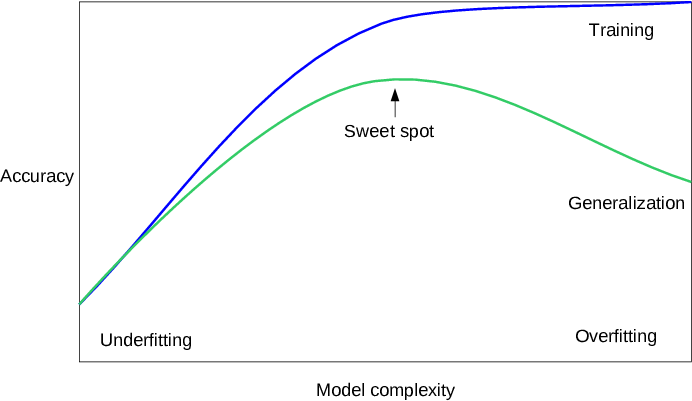
\includegraphics[width=0.6\linewidth]{figs/overfitting_underfitting_cartoon.png}
    \tiny{\href{https://github.com/amueller/introduction_to_ml_with_python/blob/master/02-supervised-learning.ipynb}{(Source)}}
\end{frame}



\section{k-Nearest Neighbors}
\subsection{k-NN classification}

\begin{frame}{k-Nearest Neighbors}{k-NN classification (I)}

     k-NN (k-Nearest Neighbors): Likely, the simplest classifier
	\begin{itemize}
		\item Given a data point, it takes its $k$ closests neighbors
		\item Same prediction than its neighbors
	\end{itemize}

    \begin{columns}
 	   \column{.40\textwidth}
        \centering 1-NN\\
	        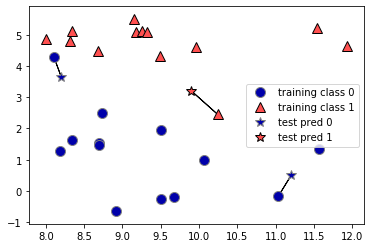
\includegraphics[width=\textwidth]{figs/1-nn.png}
 	   \column{.40\textwidth}
         \centering   3-NN\\
	        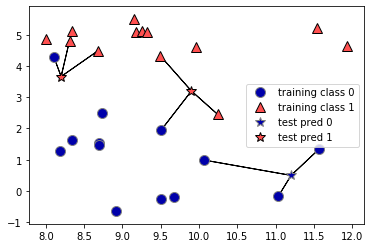
\includegraphics[width=\textwidth]{figs/3-nn.png}
    \end{columns}

    k-NN does not generate a model
    \begin{itemize}
		\item The whole dataset must be stored
	\end{itemize}
    $k$ uses to be an odd number (1-NN, 3-NN, 5-NN, ...)
\end{frame}

\begin{frame}{k-Nearest Neighbors}{k-NN classification (II)}
    \centering 
	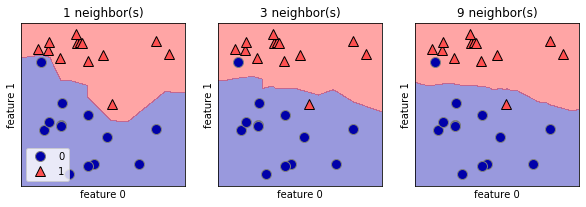
\includegraphics[width=0.7\textwidth]{figs/knnboundary.png}

    \flushleft

    $k$ determines the model complexity
    \begin{itemize}
        \item Smoother boundaries in larger $k$ values
        \item Model complexity decreases with $k$
        \item If $k$ equals the number of samples, k-NN always predicts the most frequent class
    \end{itemize}
    How to figure out the best $k$?
\end{frame}

\begin{frame}{k-Nearest Neighbors}{k-NN classification (III)}
    \centering 
	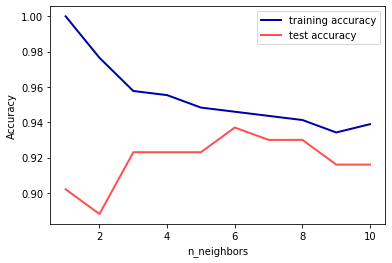
\includegraphics[width=0.5\textwidth]{figs/k-complexity.png}
\end{frame}

\IfStrEq{\modo}{muii}{
    \subsection{Scikit-Learn}

    \begin{frame}{k-Nearest Neighbors classifier}{Scikit-learn}
        \begin{exampleblock}{\texttt{sklearn.neighbors.KNeighborsClassifier}}
         \medskip

         \begin{columns}[T]
 	        \column{.01\textwidth}
 	        \column{.49\textwidth}
                Constructor arguments:
                \begin{itemize}
                    \item \texttt{n\_neighbors}: int, default=5
                    \item \texttt{metric}: string, default='minkowski'
                    \item \texttt{p}: int, default=2 ($p=1$ Manhatan distance, $p=2$ euclidean distance)
                \end{itemize}

 	        \column{.49\textwidth}
                Attributes:
                \begin{itemize}
                    \item \texttt{classes\_}: ndarray (n\_samples)
                \end{itemize}
            \end{columns}

            \medskip

            Methods: \texttt{fit()}, \texttt{predict()}
        \end{exampleblock}

        \medskip

        \centering \href{https://scikit-learn.org/stable/modules/generated/sklearn.neighbors.KNeighborsClassifier.html}{(Scikit-Learn reference)}

    \end{frame}
}{}



\subsection{kNN regression}

\begin{frame}{k-Nearest Neighbors}{kNN regression (I)}
    \begin{columns}
 	   \column{.50\textwidth}
        \begin{block}{k-NN regression}
         Given a data point
        \begin{enumerate}
            \item Take the $k$ closest data points
            \item Predict same target value (1-NN) or averate target value (k-NN)
        \end{enumerate}
        \end{block}

        Performace is measured with a regression metric, by default, $R^2$

 	   \column{.40\textwidth}
        \centering 1-NN\\
	        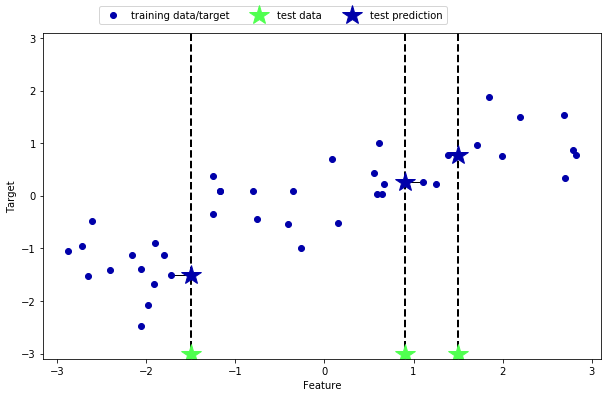
\includegraphics[width=\textwidth]{figs/1-nn-reg.png}
         \centering   3-NN\\
	        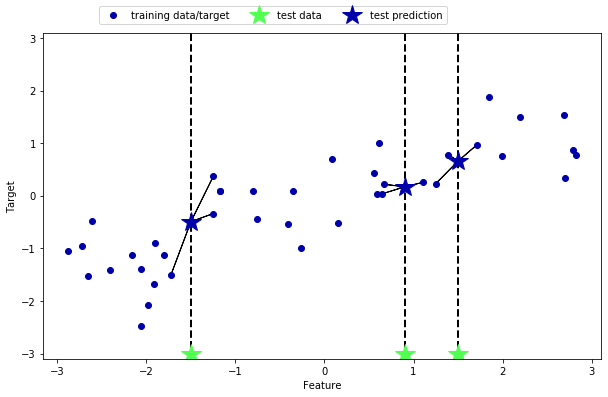
\includegraphics[width=\textwidth]{figs/3-nn-reg.png}
    \end{columns}
\end{frame}

\begin{frame}{k-Nearest Neighbors}{kNN regression (II)}
    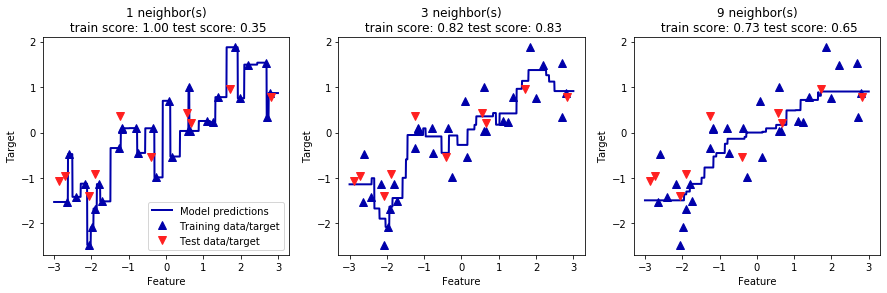
\includegraphics[width=\textwidth]{figs/knn-boundary-reg.png}

    $k$ determines boundary smoothness
    \begin{enumerate}
        \item With $k=1$, prediction visits all data points
        \item With large $k$ values, fit is worse
    \end{enumerate}
\end{frame}


\IfStrEq{\modo}{muii}{
    \subsection{Scikit-Learn}

    \begin{frame}{k-Nearest Neighbors regressor}{Scikit-learn}
        \begin{exampleblock}{\texttt{sklearn.neighbors.KNeighborsRegressor}}
         \medskip

         \begin{columns}[T]
 	        \column{.01\textwidth}
 	        \column{.49\textwidth}
                Constructor arguments:
                \begin{itemize}
                    \item \texttt{n\_neighbors}: int, default=5
                    \item \texttt{metric}: string, default='minkowski'
                    \item \texttt{p}: int, default=2 ($p=1$ Manhatan distance, $p=2$ euclidean distance)
                \end{itemize}

 	        \column{.49\textwidth}
                Attributes:
            \end{columns}

            \medskip

            Methods: \texttt{fit()}, \texttt{predict()}
        \end{exampleblock}

        \medskip

        \centering \href{https://scikit-learn.org/stable/modules/generated/sklearn.neighbors.KNeighborsRegressor.html}{(Scikit-Learn reference)}

    \end{frame}
}{}

\subsection{Summary}
\begin{frame}{k-Nearest Neighbors}{Summary}
	\begin{center}
	\begin{tabular}{cp{3cm}p{3cm}}\hline
	 	\texttt{Hyperparameters}  & \texttt{Advantages}  & \texttt{Disadvantages} \\\hline
	 	$k$                       & Simple               & Slow with large datasets  \\
	 	Distance                  & Baseline             & Bad performance with hundreds or more attributes  \\
                                  &                      & No model \\
                                  &                      & Dataset must be stored in memory \\
	 	\hline
	\end{tabular}
	\end{center}
\end{frame}



\section{Linear models}
\subsection{Ordinary least squares}
\begin{frame}{Linear models}{Linear model (I)}
    \begin{columns}
 	   \column{.60\textwidth}
        \begin{block}{Linear model}
            $y = \beta_0 + \beta_1 x_1  + \beta_2 x_2 + \dots + \beta_n x_n$
        \end{block}
        
        for a single feature $y = \beta_0 + \beta_1 x_1$, where
        \begin{itemize}
            \item $\beta_0$ is the intercept
            \item $\beta_1$ is the slope
            \item Intepretable model
        \end{itemize}

 	   \column{.40\textwidth}
		\begin{figure}
	        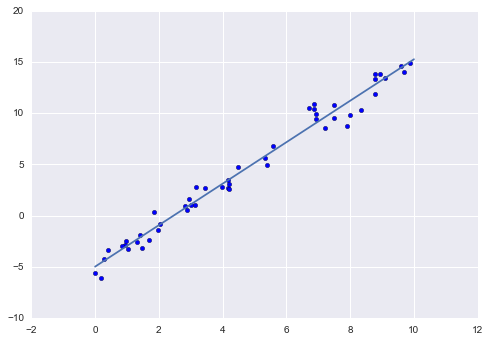
\includegraphics[width=\textwidth]{figs/regression.png}
		\end{figure}
    \end{columns}

    \bigskip

    Lineal models assume a linear relationship among variables
	\begin{itemize}
		\item This limitation can be easely overcomed
		\item Surprisingly good results in high dimensional spaces
	\end{itemize}
\end{frame}

\subsection{Linear regression}
\begin{frame}{Linear models}{Linear regression}
    Different linear models for regression
    \begin{itemize}
        \item The difference lies in how $\beta_i$ parameters are learned
    \end{itemize}

	Ordinary Least Squares (OLS): Minimizes mean squared error
	\begin{itemize}
        \item OLS does not have any hyperparameter
        \item No complexity control
        %\item Generalized Least Squares (GSL)
        %\item Weighted Least Squares (WLS)
		%\item Generalized Least Squares with AR Covariance Structure (GLSAR)
	\end{itemize}
    
    \begin{equation*}
    MSE = \frac{1}{n} \sum_{i=1}^n (x_i - y_i)^2
    \end{equation*}

    Linear regression can be used to fit non-linear models    
    \begin{itemize}
        \item Just adding new attributes
    \end{itemize}
\end{frame}

\subsection{Regularized linear models}
\begin{frame}{Linear models}{Regularized linear models}
	\alert{Regularization}: Term that penalizes complexity
	\begin{itemize}
		\item Added to the cost function
        \item Lineal models remain the same
        \item Train to minimize cost function and coefficients
        \item Intercepts are not part of regularization
	\end{itemize}

    Three regularizations
	\begin{itemize}
		\item L1 (Lasso regression),  L2 (Ridge regression) and ElasticNet (L1 and L2)
	\end{itemize}

    \begin{columns}
 	   \column{.2\textwidth}
    		\begin{block}{Lasso (L1)}
            	$\alpha \sum_j^n |\beta_j|$
        	\end{block}

	   \column{.2\textwidth}
     		\begin{block}{Ridge (L2)}
            	$\frac{\alpha}{2} \sum_j^n \beta_j^2$
        	\end{block}

	   \column{.5\textwidth}
     		\begin{block}{ElasticNet}
			$\alpha \left( \frac{\lambda}{2} \sum_j^n \beta_j^2 + (1-\lambda) \sum_j^n |\beta_j| \right)$
        	\end{block}
    \end{columns}
\end{frame}

\subsection{Ridge regression}
\begin{frame}{Linear models}{Ridge regression}
	Ridge regression (or L2 regularization) adds a new term to cost function
    \begin{equation*}
        MSE + \alpha \sum_{i=1}^n \beta_i^2
    \end{equation*}
    $\alpha$ controls the model complexity
	\begin{itemize}
		\item If $\alpha = 0$ Ridge becomes a regular linear regression
        \item Optimal $\alpha$ depends on the problem
	\end{itemize}
    Ridge by default
\end{frame}

\subsection{Lasso regression}
\begin{frame}{Linear models}{Lasso regression (I)}
	Lasso regression (or L1 regularization) adds a new term to cost function
    \begin{equation*}
        MSE + \alpha \frac{1}{2} \sum_{i=1}^n |\beta_i|
    \end{equation*}
    $\alpha$ controls the model complexity
	\begin{itemize}
		\item If $\alpha = 0$ Ridge becomes a regular linear regression
        \item Optimal $\alpha$ depends on the problem
	\end{itemize}

    Some coefficiets may be exactly zero
    \begin{itemize}
        \item Implicit feature selection
        \item Easier interpretation
        \item Better with large number of attributes
    \end{itemize}
\end{frame}

\begin{frame}{Linear models}{Lasso regression (II)}
    \centering 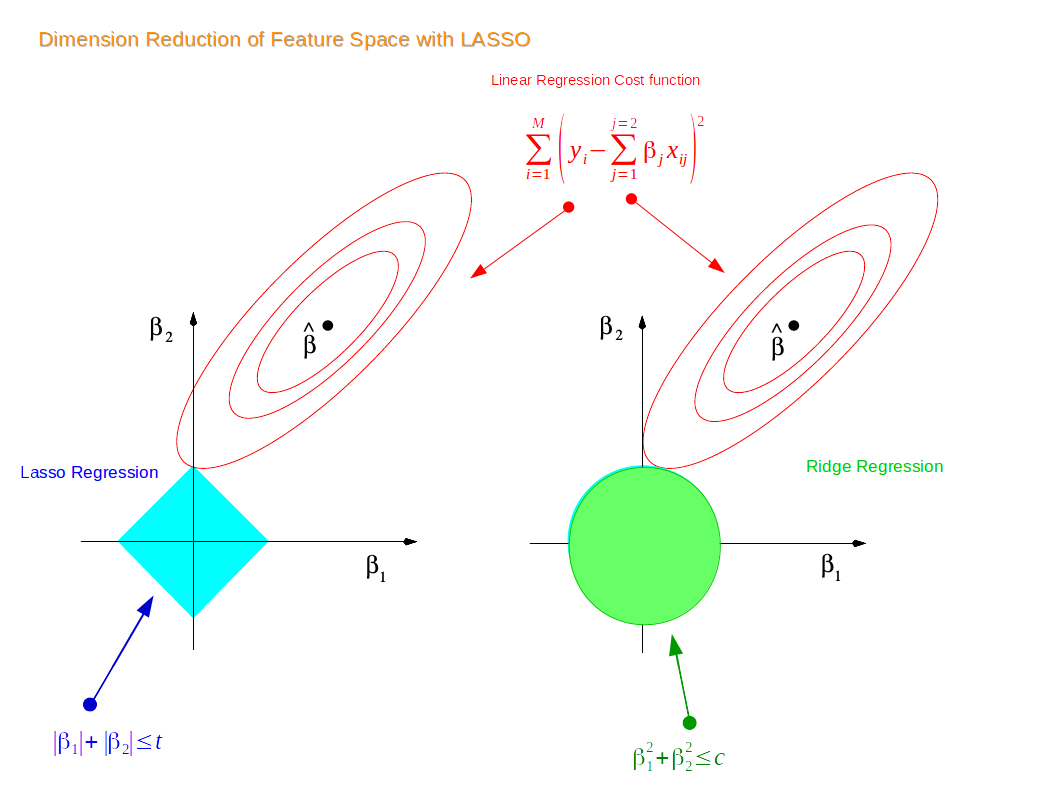
\includegraphics[width=0.7\linewidth]{figs/lasso-ridge.png}\\
    \tiny{\href{https://towardsdatascience.com/ridge-and-lasso-regression-a-complete-guide-with-python-scikit-learn-e20e34bcbf0b}{(Source)}}
\end{frame}

\subsection{ElasticNet}
\begin{frame}{Linear models}{ElasticNet}
	Lasso and Ridge can be combined
    \begin{equation*}
        MSE + \alpha \left( \lambda \frac{1}{2} \sum_{i=1}^n |\beta_i| + (1-\lambda) \sum_{i=1}^n \beta_i^2 \right)
    \end{equation*}
    Two hyperparameters
	\begin{itemize}
        \item $\alpha$ controls the model complexity
		\item $\lambda$ balances between L1 and L2
	\end{itemize}
\end{frame}

\subsection{Regularized linear models comparison}
\begin{frame}{Linear models}{Regularized linear models comparison}
    \centering
    Ridge - L2\\
    \centering 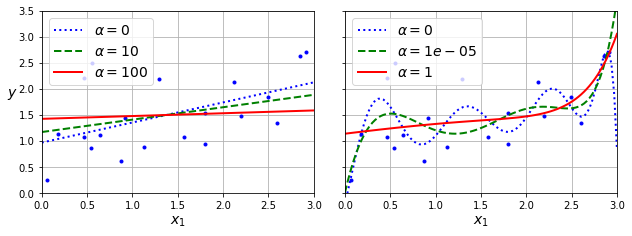
\includegraphics[width=0.7\linewidth]{figs/ridge.png}\\
    Lasso - L1\\
    \centering 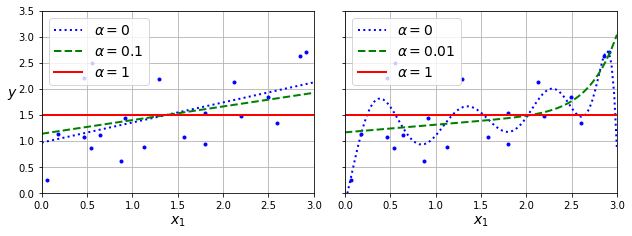
\includegraphics[width=0.7\linewidth]{figs/lasso.png}
\end{frame}

\IfStrEq{\modo}{muii}{
    \subsection{Scikit-Learn}

    \begin{frame}{Linear models}{Scikit-learn (I)}
        \begin{exampleblock}{\texttt{sklearn.linear\_model.LinearRegression}}
         \medskip

         \begin{columns}[T]
 	        \column{.01\textwidth}
 	        \column{.49\textwidth}
                Constructor arguments:
                \begin{itemize}
                    \item \texttt{fit\_intercept}: boolean, default=True
                \end{itemize}

 	        \column{.49\textwidth}
                Attributes:
                \begin{itemize}
                    \item \texttt{coef\_}:  ndarray (n\_features, )
                    \item \texttt{intercept\_}:  ndarray (n\_targets, )
                    \item \texttt{n\_features\_in\_}: int
                \end{itemize}
            \end{columns}

            \medskip

            Methods: \texttt{fit()}, \texttt{predict()}
        \end{exampleblock}

        \medskip

    \end{frame}

    \begin{frame}{Linear models}{Scikit-learn (II)}
        \begin{exampleblock}{\texttt{sklearn.linear\_model.Ridge}}
         \medskip

         \begin{columns}[T]
 	        \column{.01\textwidth}
 	        \column{.49\textwidth}
                Constructor arguments:
                \begin{itemize}
                    \item \texttt{fit\_intercept}: boolean, default=True
                    \item \texttt{alpha}: float, default=1.0
                \end{itemize}

 	        \column{.49\textwidth}
                Attributes:
                \begin{itemize}
                    \item \texttt{coef\_}:  ndarray (n\_features, )
                    \item \texttt{intercept\_}:  ndarray (n\_targets, )
                    \item \texttt{n\_features\_in\_}: int
                \end{itemize}
            \end{columns}

            \medskip

            Methods: \texttt{fit()}, \texttt{predict()}
        \end{exampleblock}

        \medskip

    \end{frame}

    \begin{frame}{Linear models}{Scikit-learn (IV)}
        \begin{exampleblock}{\texttt{sklearn.linear\_model.ElasticNet}}
         \medskip

         \begin{columns}[T]
 	        \column{.01\textwidth}
 	        \column{.49\textwidth}
                Constructor arguments:
                \begin{itemize}
                    \item \texttt{fit\_intercept}: boolean, default=True
                    \item \texttt{alpha}: float, default=1.0
                    \item \texttt{l1\_ratio}: float, default=0.5
                \end{itemize}

 	        \column{.49\textwidth}
                Attributes:
                \begin{itemize}
                    \item \texttt{coef\_}:  ndarray (n\_features, )
                    \item \texttt{intercept\_}:  ndarray (n\_targets, )
                    \item \texttt{n\_features\_in\_}: int
                \end{itemize}
            \end{columns}

            \medskip

            Methods: \texttt{fit()}, \texttt{predict()}
        \end{exampleblock}

        \medskip

    \end{frame}

    \begin{frame}{Linear models}{Scikit-learn (III)}
        \begin{exampleblock}{\texttt{sklearn.linear\_model.Lasso}}
         \medskip

         \begin{columns}[T]
 	        \column{.01\textwidth}
 	        \column{.49\textwidth}
                Constructor arguments:
                \begin{itemize}
                    \item \texttt{fit\_intercept}: boolean, default=True
                    \item \texttt{alpha}: float, default=1.0
                \end{itemize}

 	        \column{.49\textwidth}
                Attributes:
                \begin{itemize}
                    \item \texttt{coef\_}:  ndarray (n\_features, )
                    \item \texttt{intercept\_}:  ndarray (n\_targets, )
                    \item \texttt{n\_features\_in\_}: int
                \end{itemize}
            \end{columns}

            \medskip

            Methods: \texttt{fit()}, \texttt{predict()}
        \end{exampleblock}

        \medskip

    \end{frame}



}{}



\subsection{Linear models for classification}

\begin{frame}{Linear models}{Linear models for classification (I)}
    A linear regression can be used as classifier
	\begin{itemize}
		\item Just compare the prediction with a threshold (0, for instance)
            \begin{itemize}
                \item If $\hat{y} > 0$, assign class 1
                \item If $\hat{y} <= 0$, assign class -1
            \end{itemize}
        \item The decision boundary for any binary linal classifier is a line, plane or hyperplane
	\end{itemize}

    A \alert{logistic regression} is a generalization of a linear regression
    \begin{itemize}
        \item It is a binary classifier
        \item Its output is a probability
    \end{itemize}
    \begin{equation*}
        p = \sigma\left(\beta_0+\sum_{i=1}^{n} \beta_i x_i\right),
    \end{equation*}
    where $\sigma(t)$ is the logistic function, defined as $\sigma(t) = \frac{1}{1 + e^t}$

    \vspace{-3cm}
    \flushright
   	\begin{tikzpicture}[scale=0.4]
    	\begin{axis}[ 
        	xlabel=$x$,
          	ylabel={$g(x) = \frac{1}{1+e^{-x}}$}
      	] 
       	\addplot[mark=none, red] {1/(1+e^(-x))}; 
    	\end{axis}
	\end{tikzpicture}
\end{frame}

\begin{frame}{Linear models}{Linear models for classification (II)}
    \centering 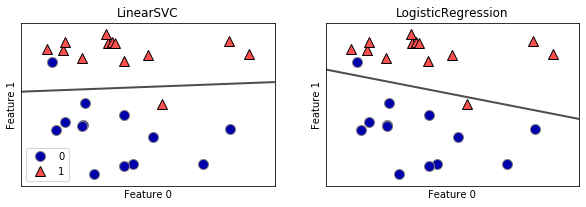
\includegraphics[width=0.8\linewidth]{figs/logistic.png}
\end{frame}

\begin{frame}{Linear models}{Linear models for classification (III)}
    \begin{columns}
 	   \column{.5\textwidth}
        The model can be regularized with L1, L2 and ElasticNet
        \begin{itemize}
            \item In Scikit-Learn, regularization strength is given by C
            \item Lower values of C correspond to smaller regularization strength
        \end{itemize}

 	   \column{.5\textwidth}
        \centering 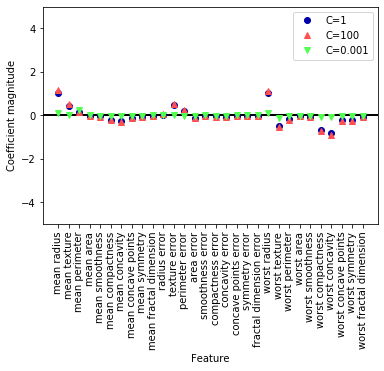
\includegraphics[width=\linewidth]{figs/logistic-c.png}
    \end{columns}
\end{frame}

\IfStrEq{\modo}{muii}{
    \subsection{Scikit-Learn}

    \begin{frame}{Linear models}{Scikit-learn}
        \begin{exampleblock}{\texttt{sklearn.linear\_model.ElasticNet}}
         \medskip

         \begin{columns}[T]
 	        \column{.01\textwidth}
 	        \column{.49\textwidth}
                Constructor arguments:
                \begin{itemize}
                    \item \texttt{penalty}: {‘l1’, ‘l2’, ‘elasticnet’, ‘none’}, default=’l2’
                    \item \texttt{fit\_intercept}: boolean, default=True
                    \item \texttt{alpha}: float, default=1.0
                    \item \texttt{l1\_ratio}: float, default=0.5
                \end{itemize}

 	        \column{.49\textwidth}
                Attributes:
                \begin{itemize}
                    \item \texttt{coef\_}:  ndarray (n\_features, )
                    \item \texttt{intercept\_}:  ndarray (n\_targets, )
                    \item \texttt{n\_features\_in\_}: int
                \end{itemize}
            \end{columns}

            \medskip

            Methods: \texttt{fit()}, \texttt{predict()}
        \end{exampleblock}

        \medskip

    \end{frame}

}{}

\subsection{Summary}
\begin{frame}{Linear models}{Summary}
	\begin{center}
	\begin{tabular}{cp{3cm}p{3cm}}\hline
	 	\texttt{Hyperparameters}  & \texttt{Advantages}  & \texttt{Disadvantages} \\\hline
	 	 -                        & Fast train and predict        & No complexity tuning  \\
	 	 $\alpha$ (L1, L2, ElasticNet) & Scales well to large datasets & Limited in low dimensional spaces  \\
	 	 $l1\_ratio$ (ElasticNet) & Better in high dimensional spaces  &   \\
	 	                          & Few hyperparameters           &   \\
	 	                          & Interpretable                 &   \\
	 	\hline
	\end{tabular}
    \end{center}

    Better when the number of features is large compared to the number of samples

\end{frame}

\section{Decision Trees}

\begin{frame}{Decision Trees}
    \begin{columns}
 	   \column{.5\textwidth}
            Decision trees are a family of algorithms for classification and regression
            \begin{itemize}
                \item They learn a tree data strucure
                \item Hierarchy of if/else questions (test, or node)
                \item Decision (terminal node or leaf)
            \end{itemize}

            Usually, datasets does not contain binary attributes
            \begin{itemize}
                \item Continous features
                \item Is feature $i$ larger than value $a$?
            \end{itemize}

 	    \column{.5\textwidth}
            \centering 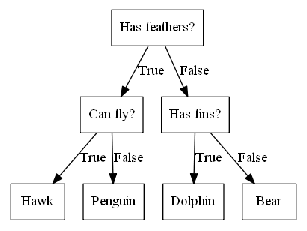
\includegraphics[width=\linewidth]{figs/tree-game.png}
    \end{columns}
\end{frame}

\subsection{Building decision trees}

\begin{frame}{Decision Trees}{Building decision trees (I)}
    \begin{columns}
 	   \column{.6\textwidth}
            %Learning a tree means learning the sequence of questions that gets the true answer most quickly

            \begin{block}{Tree learning algorithm}
                \begin{enumerate}
                    \item Begin with the root node
                    \item Searches all possible tests (according to a purity measure)
                    \item The most informative test is taken
                    \item Repeat recursively
                \end{enumerate}
            \end{block}
            Prediction of a new data point
            \begin{itemize}
                \item Classification: Majority class in the partition
                \item Regression: Average value of target values in the partition
            \end{itemize}
 	    \column{.4\textwidth}
            \centering 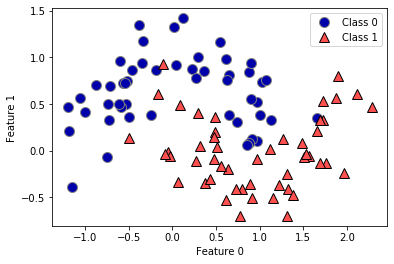
\includegraphics[width=\linewidth]{figs/tree-example.png}
    \end{columns}
\end{frame}

\begin{frame}[plain]{Decision Trees}{Building decision trees (II)}
    \begin{columns}
 	    \column{.65\textwidth}
            \centering 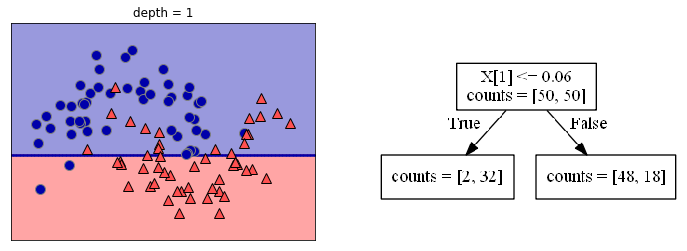
\includegraphics[width=\linewidth]{figs/tree-d1.png}
            \centering 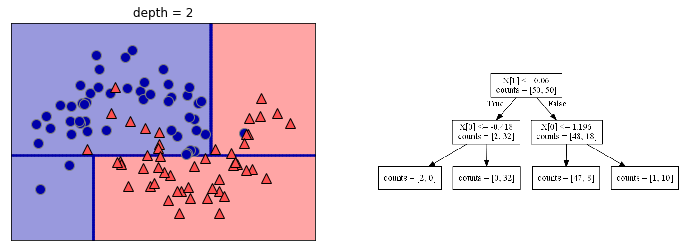
\includegraphics[width=\linewidth]{figs/tree-d2.png}
            \centering 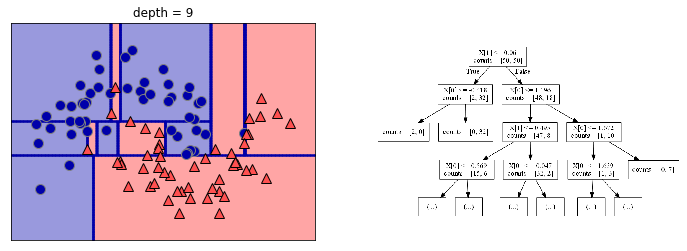
\includegraphics[width=\linewidth]{figs/tree-d9.png}
    \end{columns}
\end{frame}

\begin{frame}[plain]{Decision Trees}{Building decision trees (III)}
    Let $p_{mk}$ be the propotion of  class $k$ in node $m$, and $Q_m$ the data in node $m$

    \centering
    \bigskip

    \begin{columns}
 	    \column{.5\textwidth}
        \centering Gini \\
        \begin{equation*}
            G(Q_m) = \sum_k p_{mk} (1 - p_{ml})
        \end{equation*}

 	    \column{.5\textwidth}
        \centering Log Loss or Entropy
        \begin{equation*}
            H(Q_m) = - \sum_k p_{mk} log(p_{ml})
        \end{equation*}
    \end{columns}
\end{frame}



%\begin{frame}[plain]{Decision Trees}{Building decision trees (III)}
%    Purity measures
%    \begin{columns}
% 	    \column{.5\textwidth}
%            Gini\\
%            \begin{equation*}
%                I_G(p) = 1 - \sum_{i=1}^J p_i^2
%            \end{equation*}
%            where J is the number of classes and $p_i$ the fraction of items labeled with class $i$
%            Used in CART
% 	    \column{.5\textwidth}
%            Information gain\\
%            \begin{equation*}
%            H(T) = - \sum_{i=1}^J p_i log_2p_i
%            \end{equation*}
%            Used in ID3 and C4.5
%    \end{columns}
%\end{frame}

\subsection{Controlling complexity of decision trees}

\begin{frame}{Decision Trees}{Controlling complexity of decision trees}
    Trees tend to grow until all leaves are pure
    \begin{itemize}
        \item Very big trees in real problems
        \item Big trees use to be overfitted models
    \end{itemize}

    Two strategies to prevent overfitting 
    \begin{itemize}
        \item Pre-prunning: Stop the creation of the tree early accorgind to some criteria
            \begin{itemize}
                \item Maximum depth, number of leaves, minimum number of points in a node, ...
                \item Implemented in Sciki-Learn
            \end{itemize}
        \item Post-prunning: Build the tree and then remove nodes with little information
    \end{itemize}

            %\centering 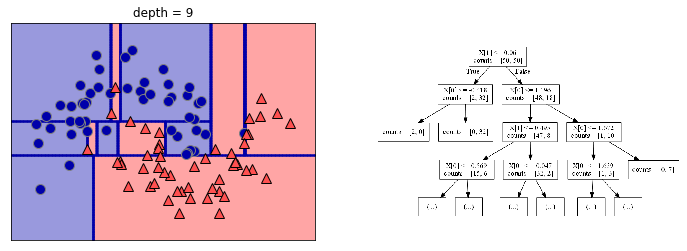
\includegraphics[width=\linewidth]{figs/tree-d9.png}
\end{frame}

\subsection{Analyzing decision trees}

\begin{frame}{Decision Trees}{Analyzing decision trees}
    Decision trees is easily explained to nonexperts
    \begin{itemize}
        \item Interpretable models
        \item Deep trees are overwhelming
        \item Trick: Observe the path with most data
    \end{itemize}

    \centering 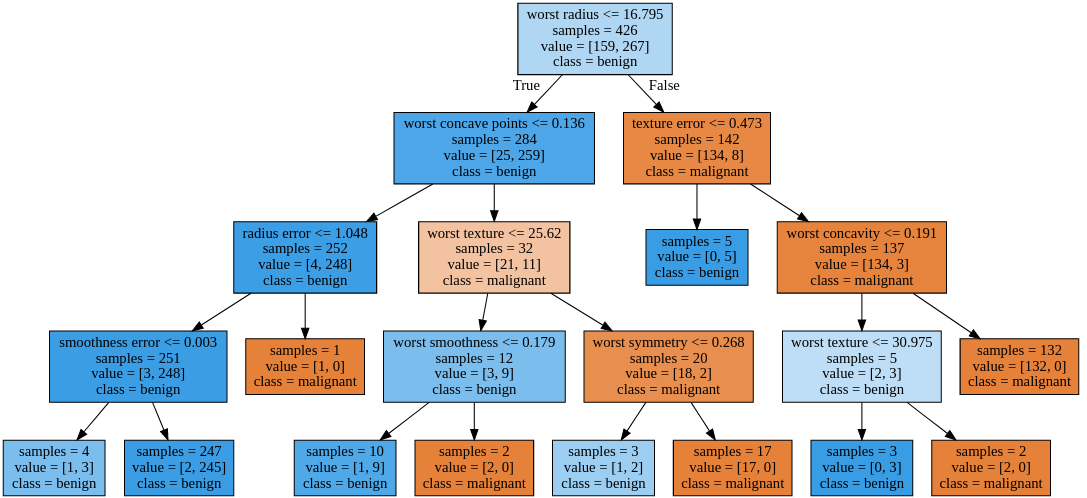
\includegraphics[width=\linewidth]{figs/tree-cancer.png}
\end{frame}

\subsection{Feature importance in trees}

\begin{frame}{Decision Trees}{Analyzing decision trees}
    \textbf{Feature importace} is a metric that summarizes features
    \begin{itemize}
        \item Number between 0 (not used at all) and 1 (perfect prediction)
        \item Feature importances sum to one
        \item Useful for feature selection and model interpretation
    \end{itemize}

   \centering 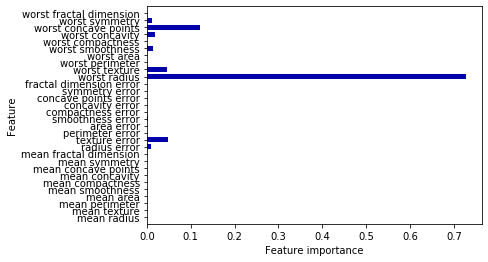
\includegraphics[width=0.5\linewidth]{figs/tree-importance.png}

   \flushleft

   \vspace{-0.5cm}

   Some considerations
   \begin{itemize}
       \item It does not inform about the relationship between attribute and target
       \item It quantifies the importance in the tree
       \begin{itemize} 
            \item Correlated attributes may score low importance
       \end{itemize}
   \end{itemize}

\end{frame}

\subsection{Decision trees in regression}

\begin{frame}{Decision Trees}{Decision trees in regression}
   \begin{columns}
      \column{.5\textwidth}
           Decision trees are not able to extrapolate
           \begin{itemize}
                \item i. e. to predict outside of the range of the training data
                \item It is specially important in regression problems
           \end{itemize}
 
     \column{.5\textwidth}
        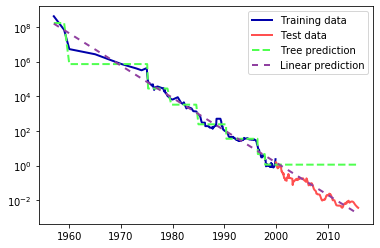
\includegraphics[width=\linewidth]{figs/tree-regression.png}
    \end{columns}
\end{frame}

\IfStrEq{\modo}{muii}{
    \subsection{Scikit-Learn}

    \begin{frame}{Decision Trees}{Scikit-learn (I)}
        \begin{exampleblock}{\texttt{sklearn.tree.DecisionTreeClassifier}}
         \medskip

         \begin{columns}[T]
 	        \column{.01\textwidth}
 	        \column{.49\textwidth}
                Constructor arguments:
                \begin{itemize}
                    \item \texttt{criterion}: {`gini', `entropy', `log\_loss'}, default=`gini'
                    \item \texttt{max\_depth}: int, default=None
                    \item \texttt{max\_leaf\_nodes}: int, default=None
                    \item \texttt{min\_samples\_leaf}: int or float, default=1
                \end{itemize}

 	        \column{.49\textwidth}
                Attributes:
                \begin{itemize}
                    \item \texttt{classes\_}: ndarray (n\_classes,)
                    \item \texttt{feature\_importances\_}: ndarray (n\_features,)
                    \item \texttt{tree\_}: Tree instance
                \end{itemize}
            \end{columns}

            \medskip

            Methods: \texttt{fit()}, \texttt{predict()}, \texttt{decision\_path()}, \texttt{get\_depth()}, \texttt{get\_n\_leaves()}
        \end{exampleblock}

        \medskip

        \centering \href{https://scikit-learn.org/stable/modules/generated/sklearn.tree.DecisionTreeClassifier.html}{(Scikit-Learn reference)}
    \end{frame}

    \begin{frame}{Decision Trees}{Scikit-learn (II)}
        \begin{exampleblock}{\texttt{sklearn.tree.DecisionTreeRegressor}}
         \medskip

         \begin{columns}[T]
 	        \column{.01\textwidth}
 	        \column{.49\textwidth}
                Constructor arguments:
                \begin{itemize}
                    \item \texttt{criterion}: {“squared\_error”, “absolute\_error”}, default=”squared\_error”
                    \item \texttt{max\_depth}: int, default=None
                    \item \texttt{max\_leaf\_nodes}: int, default=None
                    \item \texttt{min\_samples\_leaf}: int or float, default=1
                \end{itemize}

 	        \column{.49\textwidth}
                Attributes:
                \begin{itemize}
                    \item \texttt{feature\_importances\_}: ndarray (n\_features,)
                    \item \texttt{tree\_}: Tree instance
                \end{itemize}
            \end{columns}

            \medskip

            Methods: \texttt{fit()}, \texttt{predict()}, \texttt{decision\_path()}, \texttt{get\_depth()}, \texttt{get\_n\_leaves()}
        \end{exampleblock}

        \medskip

        \centering \href{https://scikit-learn.org/stable/modules/generated/sklearn.tree.DecisionTreeRegressor.html}{(Scikit-Learn reference)}
    \end{frame}
}{}

\subsection{Summary}
\begin{frame}{Decision Trees}{Summary}
	\begin{center}
	\begin{tabular}{cp{3cm}p{3cm}}\hline
	 	\texttt{Hyperparameters}  & \texttt{Advantages}  & \texttt{Disadvantages} \\\hline
	 	\texttt{max\_depth}       & Visualization        & Tend to overfit  \\
	 	\texttt{max\_leaf\_nodes} & Interpretable by non-experts     & Poor generalization  \\
	 	\texttt{min\_samples\_leaf} & Invariant to scale     &   \\
	 	\texttt{'criterion'} & Mix of categorial and numerical data     &   \\
	 	\hline
	\end{tabular}
	\end{center}
\end{frame}

\section{Ensembles of Decision Trees}

\begin{frame}{Ensembles of Decision Trees}
    TODO
\end{frame}

\IfStrEq{\modo}{muii}{
    \subsection{Scikit-Learn}

    \begin{frame}{Ensembles of Decision Trees}{Ensembles of Decision Trees : Scikit-learn}
        \begin{exampleblock}{\texttt{sklearn.cluster.AgglomerativeClustering}}
         \medskip

         \begin{columns}[T]
 	        \column{.01\textwidth}
 	        \column{.49\textwidth}
                Constructor arguments:
                \begin{itemize}
                    \item \texttt{linkage}: {‘ward’, ‘complete’, ‘average’, ‘single’}
                \end{itemize}

 	        \column{.49\textwidth}
                Attributes:
                \begin{itemize}
                    \item \texttt{n\_clusters}: int
                    \item \texttt{labels\_}: ndarray (n\_samples)
                \end{itemize}
            \end{columns}

            \medskip

            Methods: \texttt{fit()}, \texttt{fit\_predict()}
        \end{exampleblock}

        \medskip

        \centering \href{https://scikit-learn.org/stable/modules/generated/sklearn.cluster.AgglomerativeClustering.html}{(Scikit-Learn reference)}

    \end{frame}
}{}

\subsection{Summary}
\begin{frame}{Ensembles of Decision Trees}{Summary}
	\begin{center}
	\begin{tabular}{cp{3cm}p{3cm}}\hline
	 	\texttt{Hyperparameters}  & \texttt{Advantages}  & \texttt{Disadvantages} \\\hline
	 	                          &                               &   \\
	 	\hline
	\end{tabular}
	\end{center}
\end{frame}

\section{Support Vector Machines}

\begin{frame}{Support Vector Machines}
    TODO
\end{frame}

\subsection{Kernelized Support Vector Machines}
\begin{frame}{Support Vector Machines}{Kernelized Support Vector Machines}
    TODO
\end{frame}

\IfStrEq{\modo}{muii}{
    \subsection{Support Vector Machines}{Scikit-Learn}

    \begin{frame}{Support Vector Machines}{Scikit-learn}
        \begin{exampleblock}{\texttt{sklearn.cluster.AgglomerativeClustering}}
         \medskip

         \begin{columns}[T]
 	        \column{.01\textwidth}
 	        \column{.49\textwidth}
                Constructor arguments:
                \begin{itemize}
                    \item \texttt{linkage}: {‘ward’, ‘complete’, ‘average’, ‘single’}
                \end{itemize}

 	        \column{.49\textwidth}
                Attributes:
                \begin{itemize}
                    \item \texttt{n\_clusters}: int
                    \item \texttt{labels\_}: ndarray (n\_samples)
                \end{itemize}
            \end{columns}

            \medskip

            Methods: \texttt{fit()}, \texttt{fit\_predict()}
        \end{exampleblock}

        \medskip

        \centering \href{https://scikit-learn.org/stable/modules/generated/sklearn.cluster.AgglomerativeClustering.html}{(Scikit-Learn reference)}

    \end{frame}
}{}

\subsection{Summary}
\begin{frame}{Support Vector Machines}{Summary}
	\begin{center}
	\begin{tabular}{cp{3cm}p{3cm}}\hline
	 	\texttt{Hyperparameters}  & \texttt{Advantages}  & \texttt{Disadvantages} \\\hline
	 	                          &                               &   \\
	 	\hline
	\end{tabular}
	\end{center}
\end{frame}






\section{A}
\subsection{b}

\begin{frame}{A}{B}
    TODO
\end{frame}

\IfStrEq{\modo}{muii}{
    \subsection{A: Scikit-Learn}

    \begin{frame}{A}{B: Scikit-learn}
        \begin{exampleblock}{\texttt{sklearn.cluster.AgglomerativeClustering}}
         \medskip

         \begin{columns}[T]
 	        \column{.01\textwidth}
 	        \column{.49\textwidth}
                Constructor arguments:
                \begin{itemize}
                    \item \texttt{linkage}: {‘ward’, ‘complete’, ‘average’, ‘single’}
                \end{itemize}

 	        \column{.49\textwidth}
                Attributes:
                \begin{itemize}
                    \item \texttt{n\_clusters}: int
                    \item \texttt{labels\_}: ndarray (n\_samples)
                \end{itemize}
            \end{columns}

            \medskip

            Methods: \texttt{fit()}, \texttt{fit\_predict()}
        \end{exampleblock}

        \medskip

        \centering \href{https://scikit-learn.org/stable/modules/generated/sklearn.cluster.AgglomerativeClustering.html}{(Scikit-Learn reference)}

    \end{frame}
}{}

\subsection{A: Summary}
\begin{frame}{A}{B: Summary}
	\begin{center}
	\begin{tabular}{cp{3cm}p{3cm}}\hline
	 	\texttt{Hyperparameters}  & \texttt{Advantages}  & \texttt{Disadvantages} \\\hline
	 	                          &                               &   \\
	 	\hline
	\end{tabular}
	\end{center}
\end{frame}






\subsection{ARIMA}
\begin{frame}{Algorithms}{ARIMA (I)}
    \begin{columns}
 	   \column{.5\textwidth}
	   AR: Autoregressive model
	    \begin{itemize}
		\item Current observation depends on the last $p$ observations
		\item Long term memory
	    \end{itemize}

	   \column{.5\textwidth}
		\begin{block}{AR(p)}
			$X_t = c+\sum_{i=1}^p \phi_i X_{t-1}+\epsilon_t$
        	\end{block}
    \end{columns}

    \smallskip

    \begin{columns}
 	   \column{.5\textwidth}
	   MA: Moving Average model
	    \begin{itemize}
		\item Current observation linearly depends on the last $q$ innovations
		\item Short term memory
	    \end{itemize}

	   \column{.5\textwidth}
		\begin{block}{MA(q)}
			$X_t =  \mu + \epsilon_t + \theta_1 \epsilon_{t-1} + ... + \theta_q \epsilon_{t-q}$
        	\end{block}
    \end{columns}

    \bigskip

    ARMA model = AR + MA
	\begin{itemize}
		\item ARMA(p, q): Two hyperparameters, p and q
	\end{itemize}

\end{frame}

\begin{frame}{Algorithms}{ARIMA (II)}
	ARIMA = AR + i + MA (AR integrated MA)
    \begin{itemize}
	\item ARIMA(p, d, q)
	\item Three integer parameters: p, q and d (in practice, low order models)
    \end{itemize}

    \centering 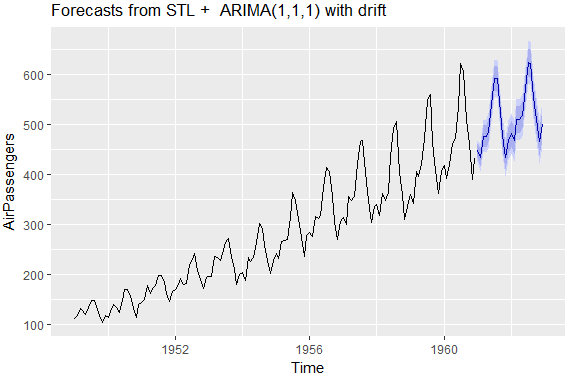
\includegraphics[width=0.6\linewidth]{figs/arima.png}

    \tiny{\href{https://itnext.io/understanding-the-forecasting-algorithm-stlf-model-29d74b3a0336?gi=282b647b24a7}{(Source)}}

    \normalsize
	\flushleft
    \alert{autoarima}: search over p, q and d
\end{frame}



\end{document}
